\documentclass{article}

\usepackage[document]{ragged2e}

\usepackage{graphicx}
\graphicspath{ {./logo/} }

\begin{document}

\begin{center}

\includegraphics[scale=0.4]{html}

\hfill

\hfill

{\huge Self-Learning HTML \& CSS}

\end{center}

\hfill

\begin{flushleft}
\textbf{\large What is the tool?}
\end{flushleft}

HTML stands for HyperText Markup Language.  It is heavily inspired by markdown, the text editing tool, and is used in conjunction with CSS to build beautiful and highly functional websites.

\hfill

\begin{flushleft}
\textbf{\large Why am I learning it?}
\end{flushleft}

I think it's a great idea to learn HTML and CSS beccause they are progrqamming institiutions.  I am reffering to the iconic history there is of these tools being the building blocks for the beginning of programmers learning journeys.

\hfill

HTML has always been at the forefront of web-development, with CSS being along for the ride,  helping developers build any sites they can imagine.

\hfill

\begin{flushleft}
\textbf{\large What is the history of HTML?}
\end{flushleft}

HTML was born on 1993, written by Tim Berners-Lee. Since then, five versions have been written, and the product of which has been seen across the entire internet, as now most sites online today are run using HTML.



\break

\begin{center}
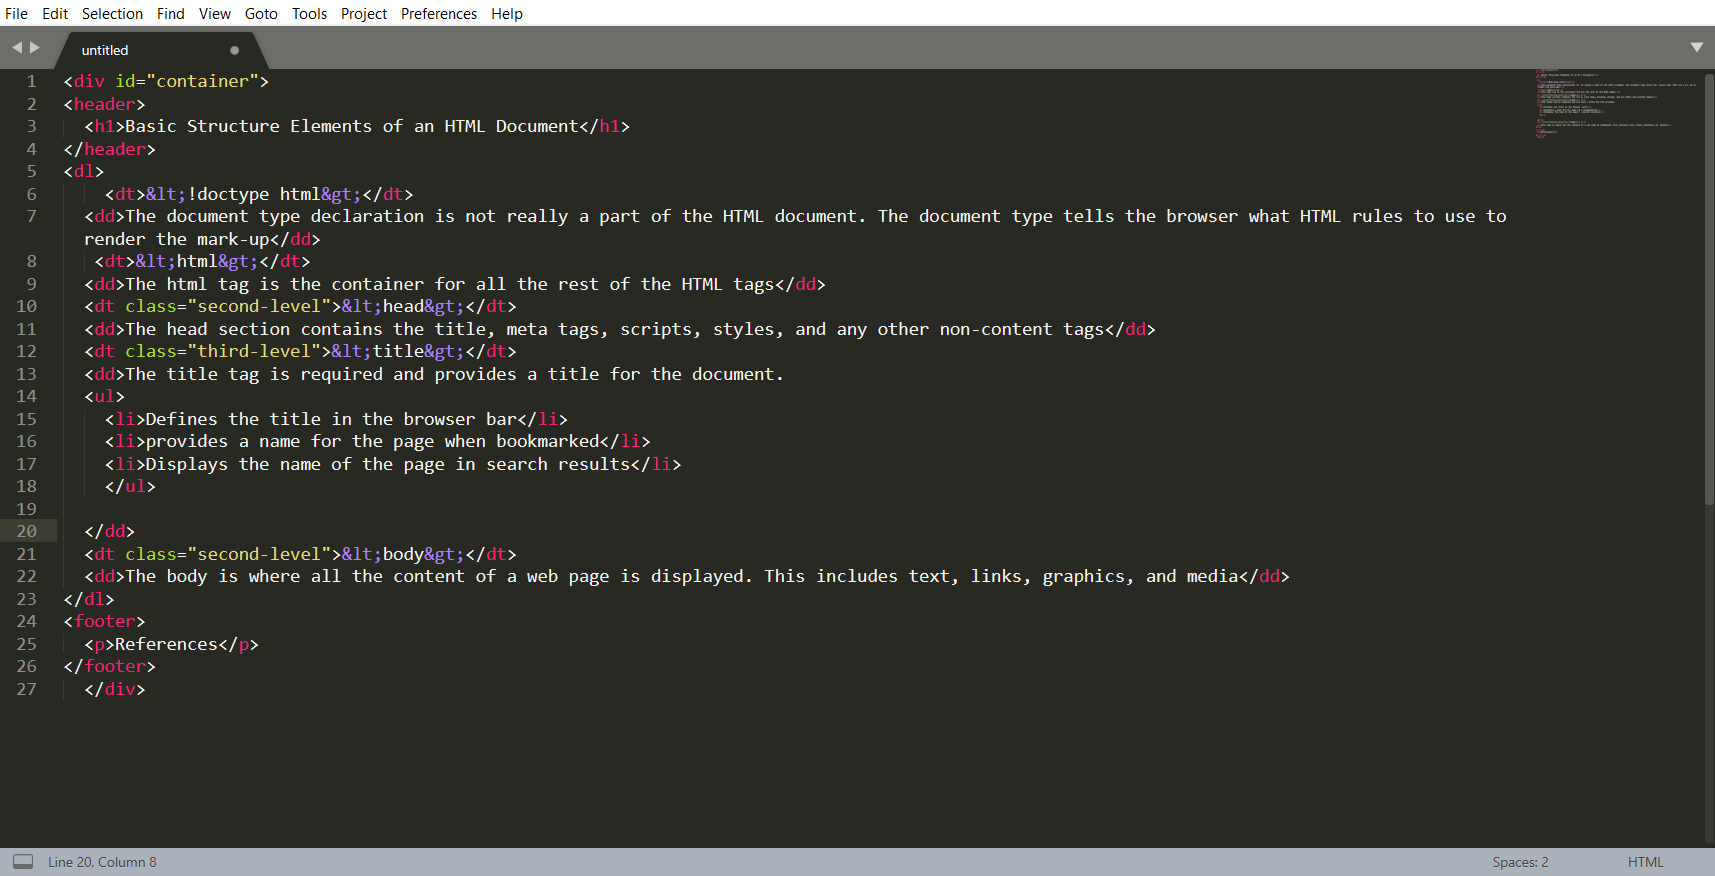
\includegraphics[scale=0.3]{code}

\hfill

Figure 1. 

This is an HTML file.  

The code is all kept inside \textless \textgreater , and sections are ended with \textless \textbackslash \textgreater

\hfill

\hfill


\includegraphics[scale=0.2]{eg}

\hfill

Figure 2. 

This is a website that has been made using HTML.  

This is just one example of many website that have been made with using the HTML and CSS languages
\end{center}

\end{document}